\documentclass[a4paper,10pt]{article}
\setlength{\parindent}{0cm}
\usepackage{amsmath, amssymb, amsthm, mathtools,pgfplots}
\usepackage{graphicx,caption}
\usepackage{verbatim}
\usepackage{venndiagram}
\usepackage[cm]{fullpage}
\usepackage{fancyhdr}
\usepackage{tikz}
\usepackage{listings}
\usepackage{color,enumerate,framed}
\usepackage{color,hyperref}
\definecolor{darkblue}{rgb}{0.0,0.0,0.5}
\hypersetup{colorlinks,breaklinks,
            linkcolor=darkblue,urlcolor=darkblue,
            anchorcolor=darkblue,citecolor=darkblue}

%\usepackage{tgadventor}
%\usepackage[nohug]{diagrams}
\usepackage[T1]{fontenc}
%\usepackage{helvet}
%\renewcommand{\familydefault}{\sfdefault}
%\usepackage{parskip}
%\usepackage{picins} %for \parpic.
%\newtheorem*{notation}{Notation}
%\newtheorem{example}{Example}[section]
%\newtheorem*{problem}{Problem}
\theoremstyle{definition}
%\newtheorem{theorem}{Theorem}
%\newtheorem*{solution}{Solution}
%\newtheorem*{definition}{Definition}
%\newtheorem{lemma}[theorem]{Lemma}
%\newtheorem{corollary}[theorem]{Corollary}
%\newtheorem{proposition}[theorem]{Proposition}
%\newtheorem*{remark}{Remark}
%\setcounter{section}{1}

\newtheorem{thm}{Theorem}[section]
\newtheorem{lemma}[thm]{Lemma}
\newtheorem{prop}[thm]{Proposition}
\newtheorem{cor}[thm]{Corollary}
\newtheorem{defn}[thm]{Definition}
\newtheorem*{examp}{Example}
\newtheorem{conj}[thm]{Conjecture}
\newtheorem{rmk}[thm]{Remark}
\newtheorem*{nte}{Note}
\newtheorem*{notat}{Notation}

%\diagramstyle[labelstyle=\scriptstyle]

\lstset{frame=tb,
  language=Oz,
  aboveskip=3mm,
  belowskip=3mm,
  showstringspaces=false,
  columns=flexible,
  basicstyle={\small\ttfamily},
  breaklines=true,
  breakatwhitespace=true,
  tabsize=3
}


\pagestyle{fancy}




\fancyhead{}
\renewcommand{\headrulewidth}{0pt}

\lfoot{\color{black!60}{\sffamily Zhangsheng Lai}}
\cfoot{\color{black!60}{\sffamily Last modified: \today}}
\rfoot{\textsc{\thepage}}



\begin{document}
\flushright{Zhangsheng Lai\\1002554}
\section*{Machine Learning: Homework 2}
\subsection*{Task 1: $K$-means}

\begin{enumerate}

\item To show that the 	algorithm terminates in finite number of steps, it suffices to show that the number of possible indicator matrix $\gamma$ is finite and the algorithm used makes $L$ a non-increasing function of the iteration. There are finite number of indicator matrix $\gamma$ as each data point can belong to exactly one cluster, thus for $n$ data points and $k$ clusters, there are $k^n$ possible configurations of the clusters. To show that $L$ is non-increasing with each iteration, it can be seen that $\gamma$ is determined by choosing the cluster $j$ such that for each data point $x_i$ for $i=1,\ldots, n$ we have $\lVert x_i-\mu_j\rVert \leq \lVert x_i-\mu_{j'}\rVert,~ \forall j'$. Now we are left to show that the recomputation of the $\mu_j$'s using the formula 
\begin{align}
\frac{\sum_{i=1}^{n}\gamma_{ij}x_i}{\sum_{i=1}^{n}\gamma_{ij}}\label{eq:mean}
\end{align}
which is equal to the mean of the data points belonging to the cluster, makes $\sum_{i=1}^{n}\gamma_{ij}\lVert x_i-\mu_j\rVert^2$ the minimum. This is true since for a given $j$, 
\begin{align*}
\frac{\partial}{\partial \mu_j}\sum_{i=1}^{n}\gamma_{ij}\lVert x_i-\mu_j\rVert^2 = -2 \sum_{i=1}^{n}\gamma_{ij} (x_i-\mu_j) 
\end{align*}
and solving for the value of $\mu_j$ when we equate the equation above to 0 gives (\ref{eq:mean}), the average of the data points in cluster $j$.

\item
\begin{align*}
\sum_{j=1}^{k}\left(\sum_{i=1}^{n}\gamma_{ij}\right)W_j(x) + nB(x) &= 
\sum_{j=1}^{k}\sum_{i=1}^{n}\gamma_{ij}\left[ \lVert x_i-\mu_j \rVert^2 + \lVert \mu_j - \widehat{x}\rVert^2\right]\\
&= 
\sum_{j=1}^{k}\sum_{i=1}^{n}\gamma_{ij}\left[ \lVert x_i \rVert^2+\lVert\mu_j \rVert^2 + \lVert \mu_j \rVert^2 + \lVert\hat{x}\rVert^2 - 2x_i^{\mathsf{T}}\mu_j - 2\mu_j^{\mathsf{T}}\hat{x}\right]\\
&= 
\sum_{j=1}^{k}\sum_{i=1}^{n}\gamma_{ij} \lVert x_i -\hat{x} \rVert^2 + C\\
&= 
\sum_{i=1}^{n} \lVert x_i -\hat{x} \rVert^2 + C = nT(x) + C
\end{align*}
where $C = \sum_{j=1}^{k}\sum_{i=1}^{n}2x_i\hat{x} +2 \lVert \mu_j \rVert^2 - 2x_i\mu_j - 2\mu_j\hat{x} = 2n\sum_{j=1}^{k}\lVert\hat{x}-\mu_j\rVert^2$. 

From the relationship we establised above, we see that $nT(x)$ is a constant that can be represented by
\begin{align*}
nT(x) = \sum_{j=1}^{k}\left(\sum_{i=1}^{n}\gamma_{ij}\right)W_j(x) + nB(x) -2n\sum_{j=1}^{k}\lVert\hat{x}-\mu_j\rVert^2
\end{align*}
Thus when the intra-cluster deviation is minimized, we need to corresponding maximize the inter-cluster deviation to keep $nT(x)$ constant.

% + C$ is a constant for fixed $\{\mu_1,\ldots, \mu_k\}$. Thus, when we try to minimize intra-cluster deviation, $W_j(x)$, we obtain new $\mu_j$'s with $W_j(x) \geq W_j(x)'$ where $W_j(x)'$ is the intra-cluster deviation with new $\mu_j$'s. Thus 


\item Let $k$ be given and assume that we have the indicator matrix $\gamma$ and the means of the clusters $\{\mu_1,\ldots,\mu_k\}$ such that $L(\gamma, \mu_1,\ldots, \mu_k)$ is a minimum. Now suppose we increase the number of clusters to $k+1$, and we initialize a new cluster mean $\mu_{k+1}$. Here we can assume that this newly added cluster mean will have a new point in its cluster when an iteration of the algorithm is being performed, otherwise, this newly added cluster will be removed the moment it is added. This means there exists a data point $x_a$ where $1\leq a \leq n$  such that 
\begin{align*}
\lVert x_a - \mu_j\rVert \geq \lVert x_a - \mu_{k+1}\rVert
\end{align*}
for all $j = 1, \ldots, k$. Thus this implies that we get 
\begin{align*}
\min_{\gamma', \mu_1, \ldots, \mu_{k+1}}L(\gamma', \mu_1, \ldots, \mu_{k+1}) \leq L(\gamma', \mu_1, \ldots, \mu_{k+1}) \leq \min_{\gamma, \mu_1, \ldots, \mu_{k}}L(\gamma, \mu_1, \ldots, \mu_{k}) 
\end{align*}
where $\gamma'$ is the new clustering with at least one point in the newly added cluster. Thus ifwe try to choose the number of clusters by minimizing $L$, $L$ will converge to zero with $n$ clusters for the $n$ data points, which is the trivial clustering of each data point into a single cluster. 

\end{enumerate}

\subsection*{Task 2: Support Vector Machine}


\begin{enumerate}
\item
\begin{figure}[h]
\centering
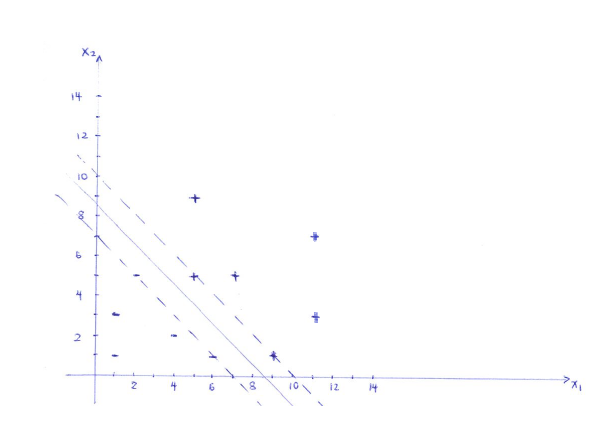
\includegraphics[width=\textwidth]{svm.png}
\end{figure}
The support vectors are $(2,5),(6,1),(5,5),(9,1)$.

\item The separating hyperplane has the formula $x_1+x_2 -8.5=0$. Thus $w_1=1$, $w_2=1$ and $b=8.5$.

\item The scaled values are $w_1 = 2/3$, $w_2=2/3$ and $b=-17/3$. We see that the division of the formula is just doing a scalar multiplication of the whole equation by $2/3$. As linear equations are unique up to scalar multiplication, we can just choose the function to be represented by the one such that the values of the support vectors are -1 and +1.


\item 
Using $f(x_1,x_2) = \frac{2}{3}x_1+\frac{2}{3}x_2-\frac{17}{3}$, \\
Functional margin for $((4,2),-1)$: $-1(17/3-(2/3\cdot 4)-(2/3 \cdot 2))=5/3$\\
Geometric margin for $((4,2),-1)$: $-5/3\div \sqrt{(-2/3)^2+(-2/3)^2} = 5\sqrt{2}/4$\\

The sign of the functional margin tells us if the classification of the point agree with the label, i.e. when the functional margin is positive, it means that the label and the classification of the point agree with each other. If the functional margin is negative, it means that the label and the classification of the point disagree with each other. The magnitude of the functional margin is the scaled value of the geometric margin.
\end{enumerate}

\end{document}